\section{Computational Modeling}\label{sec:ComputationalModeling}

Identifying the appropriate computational approach to solving a system of equations begins with a characterization of the equations. Often this can be a daunting exercise for complex models and sub-models, as is the case with this problem. The first observation about our system of equations is that they all are one dimensional in the radial direction except for the \ac{IOL} model. \ac{IOL} necessarily requires a poloidal consideration, which makes this model a 1.5 dimensional model. From there, the equations generally fall into two categories, either partial first order, non-linear, differential equations or algebraic. \prettyref{tab:DiffEqCategorization} shows the differential equations and their categorization while \prettyref{tab:AlgebraicCategorization} lists the algebraic ones. Because the equations are non-linear, the solution algorithms must be iterative in nature. The primary solver that will be explored is the Broyden solver, which is a variant within the family of Newton-Raphson solvers. The solver is discussed in \prettyref{sub:SolverSelection}.

\renewcommand\arraystretch{1.5}
\newcolumntype{L}[1]{>{\raggedright\arraybackslash}m{#1}}
\newcolumntype{C}[1]{>{\centering\arraybackslash}m{#1}}
\newcolumntype{R}[1]{>{\raggedleft\arraybackslash}m{#1}}

\begin{table}
\centering
\caption{Categorization of Differential Equations}
\begin{tabular}{|L{0.2\linewidth}|C{0.1\linewidth}|c|c|p{0.35\linewidth}|}
	\hline
	Equation & Number &Order & Type & Reason \\
	\hline
	Particle Conservation & \ref{eqn:Continuity} & 1st & Non-linear & \ac{IOL} Coefficient on $\Gamma$ is a function of $\Gamma$ vicariously through the Temperature \\
	\hline
	Energy & \ref{eqn:EnergyIon} \& \ref{eqn:EnergyElectron} & 1st & Non-linear & \ac{IOL} Coefficient on $\Gamma$ is a function of $\Gamma$ vicariously through the Temperature \\
	\hline
	Conduction Closure & \ref{eqn:ConductionIon} \& \ref{eqn:ConductionElectron} & 1st & Non-linear & Temperature multiplied by $\Gamma$ \\
	\hline
\end{tabular}
\label{tab:DiffEqCategorization}
\end{table}

\begin{table}
	\centering
	\caption{List of Algebraic Equations}
	\begin{tabular}{|l|c|}
		\hline
		Equation & Number \\
		\hline
		Minimum Energy & \ref{eqn:IOLMinV0} \& \ref{eqn:IOLEmin} \\
		\hline
		Radial Momentum & \ref{eqn:ConservationOfMomentumRadial} \\
		\hline
		Toroidal Momentum & \ref{eqn:ConservationMomentumToroidal} \\
		\hline
		Poloidal Momentum & \ref{eqn:ConservationOfMomentumPoloidal} \\
		\hline
		Beam Cross-section & \ref{eqn:beamxsection} \\
		\hline
	\end{tabular}
	\label{tab:AlgebraicCategorization}
\end{table}

\subsection{Iteration Strategy} \label{sub:CalculationOrder}

The iteration strategy requires that consideration be made for calculation order. Identifying what parameters to initialize and which ones to solve for require thought. From the initial guessed parameters, the sequence of calculations should progress in such a way that all subsequent equations have the necessary input to avoid the nefarious "use-before-calculate". The flow chart in \prettyref{fig:flowchart} shows the iteration strategy chosen. The easiest way to understand the chart is to begin with the error term $\Delta T_i$. Essentially, there are two manners by which to arrive at the ion temperature. The upper half of the flow-map utilizes an initial guess of densities, both primary ion and impurity as well as electron temperature, to source the conservation of momentum and the Beam Cross-section/Deposition calculations. Combining these with the results of the Particle conservation results in a calculation of pressure which then implies a temperature through the ideal gas law.

The second path on the lower half of the flow chart determines a temperature by way of a thermal \ac{IOL} and a fast \ac{IOL} calculation, which then feeds the conservation of energy and conduction closure equations. This results in a separate temperature. The iteration then proceeds from the error in ion temperature. The solver, of which ever flavor eventually chosen, must intelligently update the primary ion density until a solution is found.

The impurity density in this iteration strategy is assumed to be specified, since this study does not consider mechanisms of impurity source generation.

It is also worth noting that the conservation of momentum calculation was ordered the way that it is, because the poloidal and toroidal momentum equations have:
\begin{itemize}
	\item calculated particle flux, $\Gamma$ from particle conservation, 
	\item toroidal $E_\varphi^A$ and poloidal $E_\theta^A$ electric fields, which are user specified,
	\item calculated \ac{IOL} momentum contributions, and
	\item user specified \ac{NBI} momentum contributions
\end{itemize}

\begin{sidewaysfigure}[ht]
	\centering
	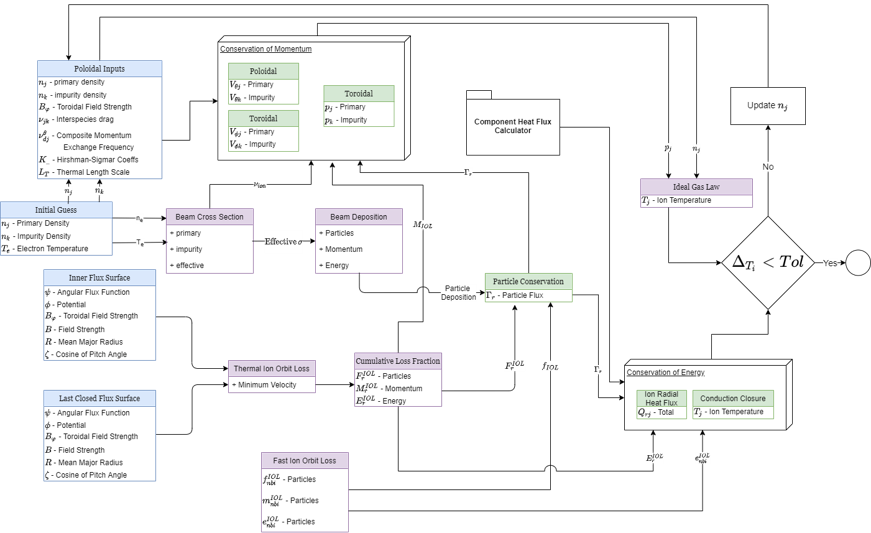
\includegraphics[width=\textwidth]{images/IterationFlowChart}
	\caption[Flow Chart]{Iteration Strategy Flow Chart}
	\label{fig:flowchart}
\end{sidewaysfigure}

\subsection{Solver Selection} \label{sub:SolverSelection}

Algebraic solvers, such as Gauss-Jordan reduction, are applicable to predictive calculations where the densities and temperatures are sourced by experimental data, but they are not applicable to boundary valued iterative problems. 
Of the solvers that appropriate for iterative techniques, several but were considered and dismissed. \acf{GMRES} style solvers are appropriate for a non-symmetric system of linear equations \cite{Kelley1995}. Our equations are non-linear. Pure Newton Methods were dismissed because they require analytic functions so that the Jacobian can be analytically calculated. Our equations do not have an obvious analytic form. That leaves us with quasi Newton-Raphson methods in which the Jacobian is calculated computationally. The most widely used quasi Newton-Raphson method is the Broyden method. The Broyden method approaches the rate of convergence of a pure Newton-Raphson method, however, it accomplishes this at a fraction of the computational cost because the full Jacobian is not recalculated, but is evaluated numerically and algorithmically updated in subsequent iterations.

The update of values from iteration to iteration follows a similar approach to Newton's methods (\cref{eqn:BroydenUpdate}), namely:
%
\begin{equation}
	x_{+} = x_c - B_c^{-1} F(x_c).
	\label{eqn:BroydenUpdate}
\end{equation}
%
This nomenclature is directly borrow from reference \cite{Kelley1995}. The subscript c indicates current values, whereas the + refers to updated values. F is the function being evaluated, and B is the Broyden matrix which is the numerical analogue of the analytic Jacobian. In pure Newton's methods, the Jacobian would be recalculated for each successive iteration. However, Broyden's method utilizes a secant update approach given by \cref{eqn:BroydenSecant}

\begin{equation}  \label{eqn:BroydenSecant}
	\begin{split}
		B_{+} = B_c + \cfrac{\left(y - B_c \, s) s^T\right)}{s^T s} = B_c + \cfrac{F(x_{+})s^T}{s^Ts} \\
		\text{where } y = F(x_{+}) - F(x_c) \text{ and } s = x_{+} - x_c
	\end{split}
\end{equation}

One last thing should be noted. It is unknown at this point how non-linear the system of equations are. If the \ac{IOL} proves to not be sensitive to changes in temperature, then it might be possible to revisit other iterative techniques such as \ac{GMRES}.
